%======================================================================
\chapter{Motivation}
%======================================================================
The project detailed in this report was created to generate random graphs for the purpose of training Generative Adversarial Networks (GAN) \cite{goodfellow2014generative}. Furthermore, the graphs created would be used as input data for a GAN that would translate images of graphs to a tactile writing system, more specifically braille. The fundamental basis for solving this translation is based around the idea of a Text-to-Image-to-Text GAN.

\hfill

More technically, the model would learn the meaning of a sentence and generate an image depicting the sentence. That image would then be put through a second ``captioning" network to provide captions to the generated images. The distance between the ground truth captions and generated captions is then explored to further improve the network \cite{hu2021text}. This system would use the data generation processes introduced in this paper as a basis for the text inputted into the system, as well as the regeneration pipeline for further image validation. The details of which will not be further brushed upon in this paper, however, it should be noted that the network will be completed by a graduate student under the same supervisor, Dr. Majid Komeili.

%----------------------------------------------------

\section{Problem Domain}
One of the issues with representing scientific graphs in tactile format is understanding of what figures should be translated. The Braille Authority of North America has a diagram on this topic to dictate whether a figure is appropriate for a tactile graphic. As \autoref{figure:decision_tree} would indicate, the graphs generated in this project fall under the category of images appropriate for a tactile graphic with one condition being most notable. The condition being the node in the decision tree that inquires as to whether a reader needs the information from a map, figure, or graph to participate in discussion, answer questions, or complete a task. This shows a significant need for tacticle graph translation which is not yet widely accessible.

\begin{figure}[hbt]
    \centering
    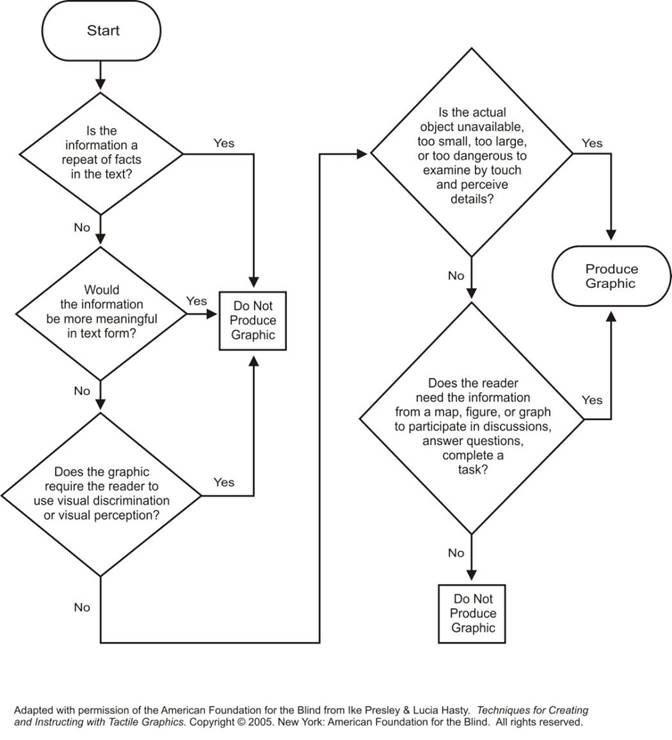
\includegraphics[width=300pt,keepaspectratio]{figures/body/motivation/decisiontree.jpg}
    \caption{A decision tree dictating whether a tactile graph is appropriate \cite{tactile_graphics}}
    \label{figure:decision_tree}
\end{figure}

%----------------------------------------------------

\section{Use Cases}
The ability to translate mathematical and scientific graphs into braille is incredibly useful. As indicated by Dr. Sile O'Modhrain from the University of Michigan, refresh-able braille displays have a wide range of problems \cite{youtube_2015}. On top of the devices being extremely costly in the range of \$3,000 - \$5,000 per line, text is only displayed one line at a time. This would be comparable to reading a book on an e-reader line by line, which is most unwelcome amongst the visually impaired \cite{youtube_2015}. The final issue, which is the underlying motivation for this problem, is that modern braille devices are unable to communicate spatially distributed information \cite{youtube_2015}. This would include bar charts, histograms, line graphs, and spreadsheets amongst others. Part of the issue comes with graph flexibility, as providing a digital medium to express a multitude of graph types is not an insignificant task.

\hfill

Currently, no accessible solution exists for effectively communicating a wide range of graphs through a tactile format like braille. While existing solutions, such as the BrailleNote Touch \cite{kendrick_2020}, have some graphing functionality (\autoref{figure:braillenote_touch}), they still face the issues of cost and flexibility mentioned above. As specified in \autoref{section:modularity}, a major developmental milestone of the project was the modularity and flexibility allowed by the graph generation pipeline. As the approach is entirely digital, the proposed approach combats all aforementioned issues with an additional benefit of accessibility as well.

\begin{figure}[hbt]
    \centering
    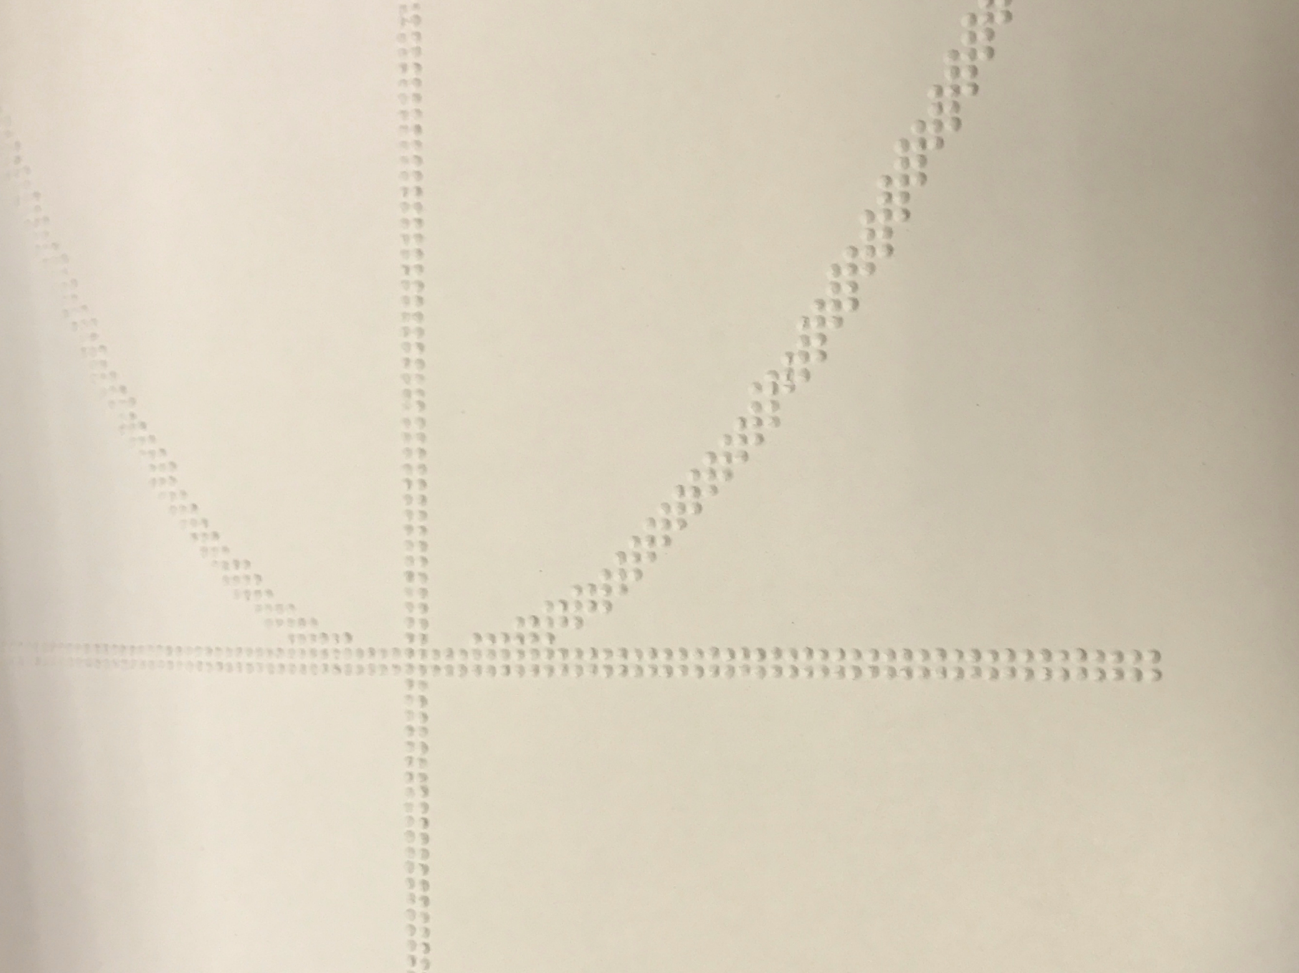
\includegraphics[width=150pt,keepaspectratio]{figures/body/motivation/braillenote_touch.png}
    \caption{Visualization of graphs in braille using the BrailleNote Touch \cite{lee_2018}}
    \label{figure:braillenote_touch}
\end{figure}

\hfill

By converting the text to an intermediary language prior to tactile representation, the language could be processed through a text-to-speech pipeline. This would be critical for assistive technologies like screen readers or Apple's VoiceOver \cite{apple_support_2020} software as information pertaining to the graphs could be relayed through a medium like English. As much of the content in today's world is absorbed through digital mediums like computers, phones, and other electronic devices, having a digital solution for graph translation would be invaluable.

\section{Existing Solutions}
While there are existing solutions for individual graph generation, such as using Gaussian distributions for a histogram, there is no widespread solution for generating random charts of varying types. Many projects use techniques such as Gaussian distribution (\autoref{subsubsection:normal_distribution}) for histogram generation and a sorted uniform distribution (\autoref{subsubsection:uniform_distribution}) for bar charts, but having a customizable approach to the entire process is hard to come by. This is especially true as most projects tend to pick a single visualization library and stick to it.

